\section{DeepPicar Overview}

\begin{figure}[h]
  \centering
  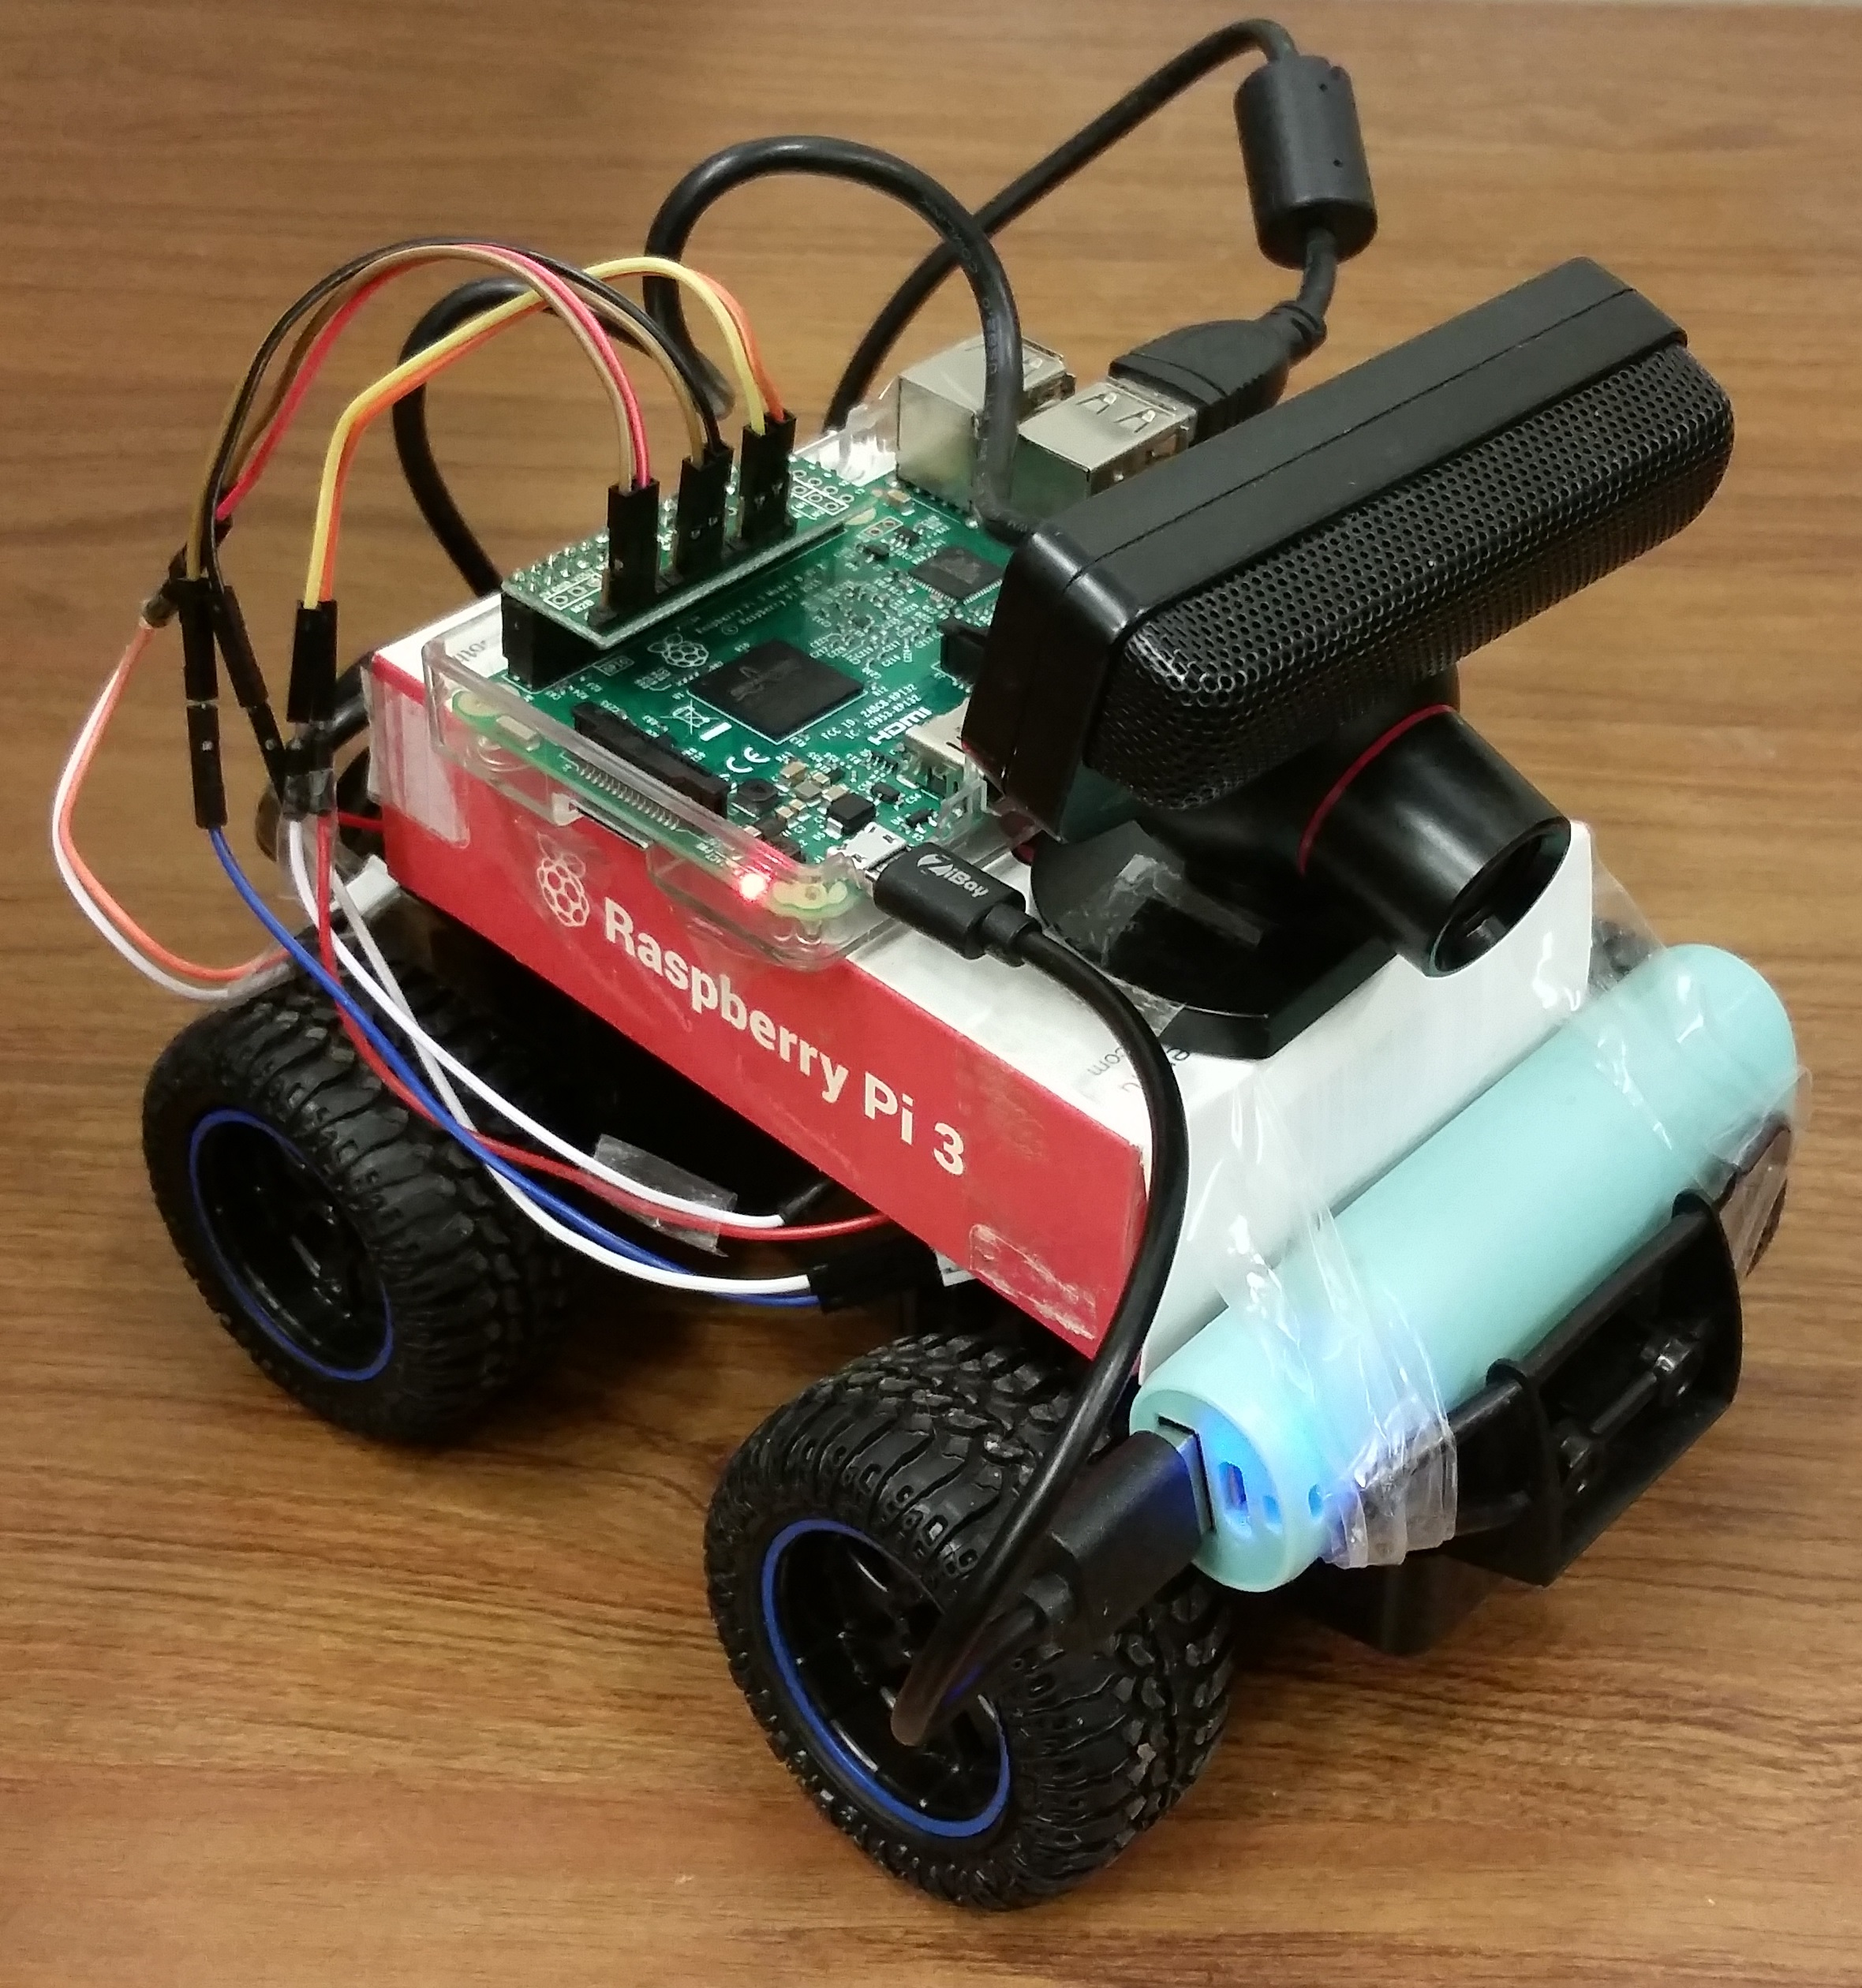
\includegraphics[width=.4\textwidth]{figs/DeepPicar_platform}
  \caption{DeepPicar platform.}
  \label{fig:overview}
\end{figure}

In this section, we provide an overview of our DeepPicar platform. In
developing DeepPicar, one of our primary goals is to replicate the
NVIDIA's DAVE-2 system on a smaller scale with using a low cost
multicore platform, Raspberry Pi 3. Because Pi 3's computing
performance is much lower than that of the DRIVE PX platform, used in
DAVE-2, we are interested in if and how we can process
computationally expensive neural network operations in
real-time. Specifically, inferencing (forward pass processing)
operation must be completed within each control period
duration---e.g., WCET of 50ms for 20Hz control frequency---locally on
the Pi 3 platform, although training of the network (back-propagation
for weight updates) can be done offline and remotely using a desktop
computer.

Figure~\ref{fig:overview} shows the DeepPicar, which is comprised of a
set of inexpensive components: a Raspberry Pi 3 Single Board Computer
(SBC), a Pololu DRV8835 motor driver, a Playstation Eye webcam, a
battery, and a 1:24 scale RC car. Table~\ref{tbl:carbom} shows
estimated cost of the system.

\begin{table}[h]
  \centering
  \begin{tabular}{|r|r|}
    \hline
    Item                    & cost (\$) \\
    \hline
    Raspberry Pi 3 Model B  & 35 \\
    New Bright 1:24 scale RC car       & 10 \\
    Playstation Eye camera  &  7 \\
    Pololu DRV8835 motor hat&  8 \\
    External battery pack \& misc.   & 10 \\
    \hline
    Total                   & 70 \\
    \hline
  \end{tabular}
  \caption{DeepPicar's bill of materials (BOM)}
  \label{tbl:carbom}
\end{table}

For the neural network architecture, we adopt a tensorflow version of
NVIDIA's DAVE-2 convolutional neural network (CNN), published by
Fridman at  MIT~\footnote{https://github.com/lexfridman/deeptesla}. As
in NVIDIA's DAVE-2, the CNN takes raw color image (200x66 RGB pixels)
as input and produce a single steering angle value as
output. Figure~\ref{fig:architecture} shows the network architecture, which
is comprised of 9 layers, 250K parameters, and about 27 million
connections.

\begin{figure}[h]
  \centering
  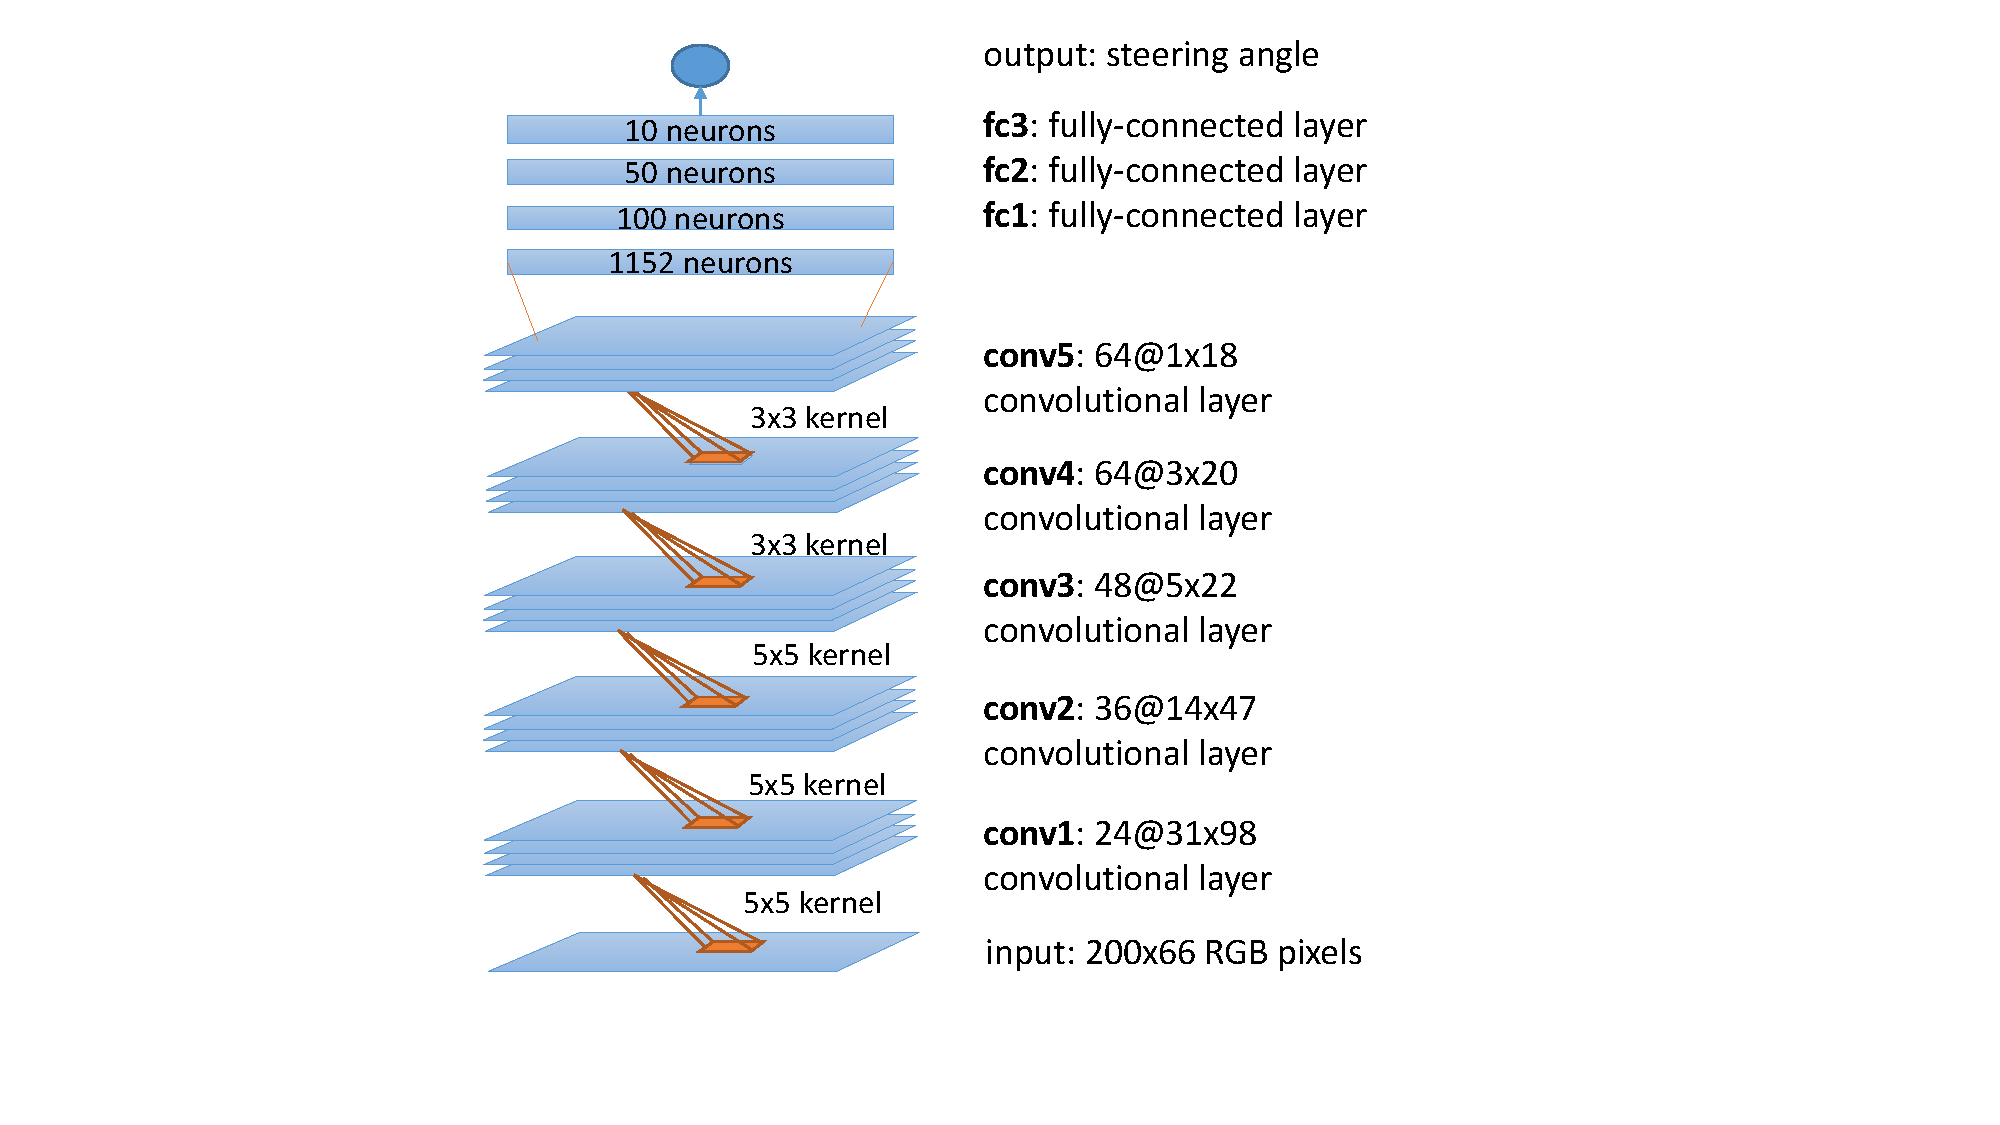
\includegraphics[width=.4\textwidth]{figs/architecture}
  \caption{DeepPicar's neural network architecture: 9 layers (5
    convolutional, 4 fully-connected layers), 27 million connections,
    250K parameters. The architecture is identical to the one used
    in NVIDIA's real self-driving car~\cite{Bojarski2016}.}
  \label{fig:architecture}
\end{figure}

% data collection and training.
To collect the training data, a human pilot manually drives the RC car
on a small track we created (Figure~\ref{fig:track}) to record
timestamped video and contol commands. The stored data is then copied 
to a desktop computer, which equips a NVIDIA GTX 1060 GPU, where we
train the network to accerate training speed. 
For comparison, training the network on the Raspbeery Pi 3 takes
approximately 4 hours, whereas it takes only about 5 minutes on the
desktop computer using the GTX 1060 GPU.

\begin{figure}[h]
  \centering
  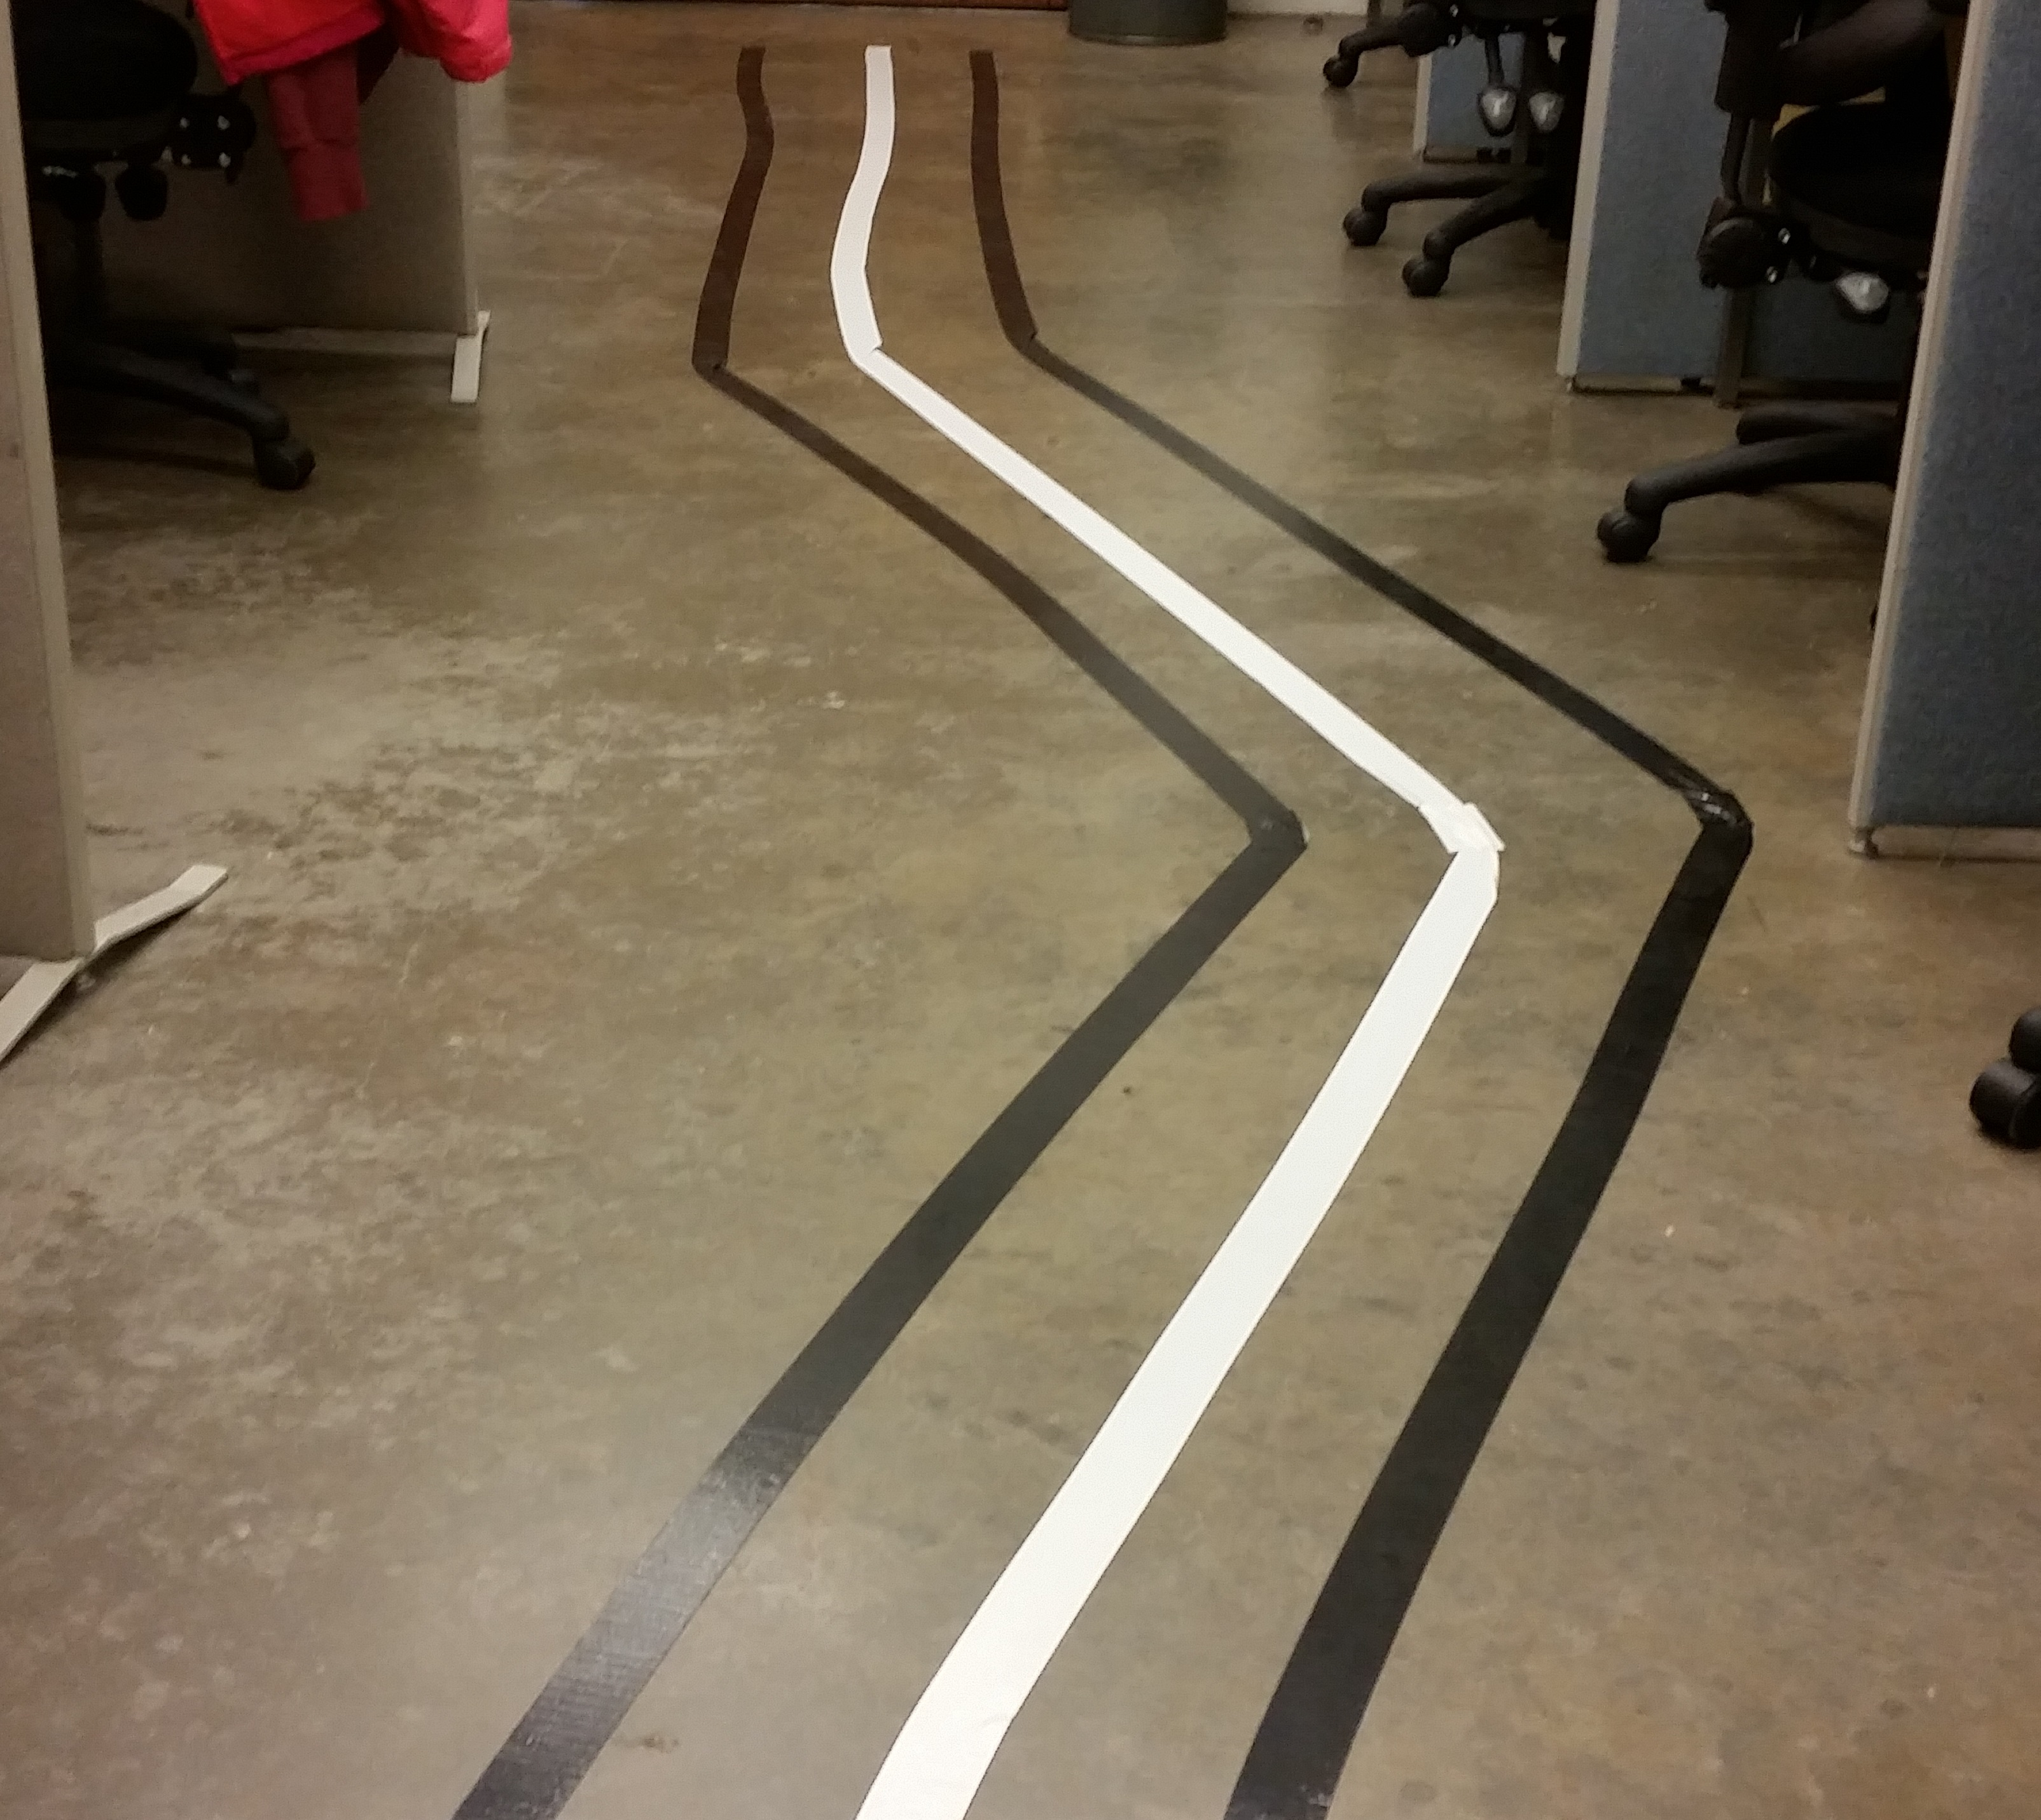
\includegraphics[width=.4\textwidth]{figs/track_new2}
  \caption{One of the custom tracks used for training/testing.}
  \label{fig:track}
\end{figure}


% inferencing on pi3
Once the network is trained on the desktop computer, the trained model
is copied back to the Raspberry Pi computer. The network is then used
by the car's main controller, which feeds a image frame from the web
camera as input to the network. The produced steering angle output is
then converted as the PWM value of the steering motor of the
car. Figure~\ref{fig:controlloop} shows simplified psuedo code of the
controller's main loop. Among the five steps, step 3---network
inferencing---is most computationally intensive and dominates the
execution time.

\begin{figure}[t]
   \lstset{language=python,
           basicstyle=\ttfamily\small,
           keywordstyle=\color{blue}\ttfamily,
           stringstyle=\color{red}\ttfamily,
           commentstyle=\color{green}\ttfamily
          }  
  \lstinputlisting[language=python]{control.py}
  \caption{Control loop}
  \label{fig:controlloop}
\end{figure}

Note that although the steering angle output of the network $angle$ is
a continuous real value, the RC car platform we used unfortunately
only supports three discrete angles---left (-30$^{\circ}$), center
(0$^{\circ}$), and right (+30$^{\circ}$)---as control
inputs. Currently, we approximate the network generated real-valued
angle to the closest one of the three angles, which may
introduce inaccuracy in control.
In the future, we plan to use different (more expensive) RC car
platforms that can precisely control the car's steering angle. We
would like to stress, however, that the use of different RC car
platforms has no impact in terms of computational 
aspects of the system, and that our main focus of this study is
not in improving network accuracy but in closely replicating the
DAVE-2's network architecture and its real-time characteristics.

Nevertheless, the trained models were still able to achieve reasonable
a degree of accuracy, successfully navigating several different tracks 
we trained. The source code, build instruction, and a collection of
self-driving videos of the DeepPicar can be found at:
\url{https://github.com/heechul/picar}.
%% \begin{center}
%% \end{center}

%% We employ a small and relatively inexpensive RC car that is capable of
%% performing basic automotive operations. However, the car we use
%% doesn't replicate the capabilities of other autonomous vehicle
%% platforms, as it is more simplistic in nature. Notably, the RC car we
%% use only has three possible options in terms of turning: center, left,
%% and right. As such, control of the car may be less precise at times,
%% and may negatively affect performance. The car is capable of other
%% operations that aren't used within the scope of this
%% platform. Specifically, the car is able to drive in reverse and the
%% driving speed can be changed. In our experiments, we have the RC car
%% drive forward, and at a constant speed. 

%% Our platform also comes equipped with a camera that is used for both
%% recording training videos and providing input frames to the model
%% whenever the Picar is self-driving. We chose the Playstation Eye
%% Camera due to its ability to reach and maintain higher fps levels
%% while also remaining relatively low-cost. One concern, however, is the
%% affect of camera latency on the self-driving performance of our
%% platform. While humans are able to see environmental changes in
%% real-time, the same can't be said for cameras since there is a delay
%% between when frame capture by the camera, and when it is read by the
%% Raspberry Pi 3. As a result, it is possible for the model to be given
%% an input frame that is different from the real world, thus impacting
%% the performance of the Picar.

%% Compared to other existing autonomous vehicle platforms, such as the
%% F1/10 and NVIDIA DAVE-2, the Picar platform is capable of performing
%% the same operations while using more cost inexpensive components. As
%% shown by Table 1, the components selected for the Picar all cost
%% considerably less than the other  platforms when focusing on the
%% common components (camera, power supply, etc.). Including the other
%% components used in the F1/10 and DAVE-2, such as the additional
%% sensors employed by both, the difference  in cost would be even
%% greater.

%% \subsection{Model Training}
%% In order to operate the Picar as an autonomous vehicle, we utilize the
%% DeepTesla library, which is capable of training a deep neural network
%% (DNN) with end-to-end learning, that could then be used by the  Picar
%% for autonomous driving. Please note that it is more efficient to
%% execute the actual model training  process on a different system with
%% an NVIDIA GPU, rather than on the Raspberry Pi 3 itself. This is
%% because DeepTesla trains the DNN with the Tensorflow library, which
%% greatly benefits from the use of  gpu-enabled operations. For
%% comparison, training a model on the Pi took approximately 6 hours,
%% whereas  the time it took on a computer with a NVIDIA GPU was only
%% around 5 minutes!

%% We train our model on a custom made track/lane composed of black and
%% white duct tape, where the black  tape represents the bounds of the
%% track, and the white tape marks the center of the lane. The model is
%% taught to stay close to the center of the lane for as long as
%% possible, and to turn whenever it  reaches/crosses the outer lane
%% bounds so that it remains on the track. For data, we navigate and
%% record  the car going both ways across the track, and use the
%% collected videos to train the model(s) that will  be used later for
%% angle prediction while the car is self-driving.

%% \begin{table*}[h]
%%   \centering
%%   \begin{tabular} {| l | l | l | l | l |}
%%     \hline
%%     \textbf{Platform} & \textbf{Picar} & \textbf{F1/10} & \textbf{NVIDIA DAVE-2}\\ \hline  
%%     Car & Mini RC Car (\$10) & Traxxas 1/10th car platform (\$299.97) & TBD\\ \hline
%%     Embedded system & Raspberry Pi 3 Model B (\$35.00) & NVIDIA Jetson TK1 (\$192.99) & NVIDIA DRIVE PX \\ \hline
%%     CPU & Cortex A-53 quad core & Cortex A-15 quad core & 8x Cortex A-57 quad core, 8x Cortex A-53 quad core \\ \hline
%%     Camera & Playstation Eye camera (\$6.99) & ZED camera (\$449.00) & 3x cameras\\ \hline
%%     Power Supply & Mobile battery (\$5.99) & Energizer battery pack (\$159.00) & TBD\\
%%     \hline
%%   \end{tabular}
%%   \caption{Comparison of components used in autonomous vehicle platforms.}
%% \end{table*}

